%==============================================================================
% presentation.tex
%==============================================================================


%==============================================================================
% Configuration
%==============================================================================

% Internationalisation
\usepackage[utf8]{inputenc}
\usepackage[T1]{fontenc}
% \usepackage[ngerman]{babel}

% Different packages
\usepackage{url}
\usepackage{color,listings,paralist}
\usepackage{enumerate}
\usepackage{tabularx}
\usepackage{alltt}

% Use default Acrobat reader fonts
\usepackage{mathpazo}

% Use CM fonts (increases document size)
\usepackage{ae}

% Use images
\usepackage{graphicx}

% Configure beamer
\usetheme[secheader]{Ikhono}
\usefonttheme[onlylarge]{structurebold}
\setbeamertemplate{navigation symbols}{}

% Variables
\providecommand{\Title}{Parallel Programming}
\providecommand{\Subtitle}{Recitation Session 10}
\providecommand{\Author}{Thomas Weibel <weibelt@ethz.ch>}
\providecommand{\Institute}{Laboratory for Software Technology, \\
  Swiss Federal Institute of Technology Z\"urich}
\providecommand{\Date}{May 20, 2010}

% PDF settings
\hypersetup{
  pdftitle={\Title, \Subtitle},
  pdfauthor={\Author},
  pdfsubject={\Institute},
  pdfkeywords={parallel programming} 
}

% Titlepage
\title{\Title}
\subtitle{\Subtitle}
\author{\Author}
\institute{\Institute}
\date{\Date}

% Listings
\lstdefinestyle{Default}{
  language=Java,
  tabsize=2,
  mathescape=true,
  inputencoding=utf8,
  showstringspaces=false,
  fontadjust=true,
  basicstyle=\ttfamily,
  keywordstyle=\color{blue}\bfseries,
}
\lstset{style=Default}


%==============================================================================
% Document
%==============================================================================

\begin{document}


% Titlepage
\begin{frame}[plain]
  \titlepage
\end{frame}


\section*{Introduction}

\begin{frame}{Executive Summary}
  \begin{itemize}
  \item TODO
  \end{itemize}
\end{frame}


\section{MVC Revisited}

\begin{frame}{Outline}
  \tableofcontents[current]
\end{frame}

\begin{frame}{Model-View-Controller}
  TODO: Picture

  \vspace{\stretch{1}}

  \begin{description}
  \item[Direct association:] has-a relationship
  \item[Indirect association:] Observer pattern
  \end{description}
\end{frame}

\begin{frame}{Roles of Participants}
  \begin{itemize}
  \item Model:
    \begin{itemize}
    \item domain specific knowledge
    \item adds meaning to raw data
    \end{itemize}
  \item View:
    \begin{itemize}
    \item render data
    \item capture user gestures
    \end{itemize}
  \item Controller:
    \begin{itemize}
    \item respond to events 
    \item asynchronously invoke changes on model
    \end{itemize}
  \end{itemize}
\end{frame}

\section{Game of Life}

\subsection{Solution 1}

\begin{frame}{Outline}
  \tableofcontents[current]
\end{frame}

\begin{frame}{Design of Solution 1}
  \begin{itemize}
  \item \lstinline!Application! class:
    \begin{itemize}
    \item Main window and controls
    \item Create and terminate the modeling thread
    \end{itemize}
  \item \lstinline!Field! class:
    \begin{itemize}
    \item Drawing field: keeps copy of model state
    \end{itemize}
  \item \lstinline!Controller! class:
    \begin{itemize}
    \item Has data and methods that can be applied on the data
    \end{itemize}
  \end{itemize}
\end{frame}

\begin{frame}{Code}
  \begin{center}
    {\huge Let's take a look at the code}
  \end{center}
\end{frame}

\subsection{Solution 2}

\begin{frame}{Outline}
  \tableofcontents[current]
\end{frame}

\begin{frame}{Model}
  \begin{itemize}
  \item Represents grid of cells, that can be dead or alive
    \begin{itemize}
    \item[$\rightarrow$] internally private boolean array
    \end{itemize}
  \item Synchronized methods
  \item Implements computing next state of world
  \end{itemize}

  TODO: Picture
\end{frame}

\begin{frame}{View}
  TODO: Picture
\end{frame}

\begin{frame}{Controller}
  TODO: Picture
\end{frame}


\section{OpenMP}

\begin{frame}{Outline}
  \tableofcontents[current]
\end{frame}

\begin{frame}{OpenMP in a Nutshell}
  \begin{itemize}
  \item OpenMP is an API that consists of three parts
    \begin{itemize}
    \item Directive-based language extension
    \item Runtime library routines
    \item Environment variables
    \end{itemize}
  \item Three categories of language extensions
    \begin{itemize}
    \item Control structures to express \alert{parallelism}
    \item Data environment constructs to express \alert{communication}
    \item Synchronization constructs for \alert{synchronization}
    \end{itemize}
  \end{itemize}
\end{frame}

\begin{frame}{Parallel Control Structures}
  Alter flow of control in a program

  \begin{itemize}
  \item[$\rightarrow$] fork/join model
  \end{itemize}

  \vspace{\stretch{1}}

  \begin{center}
    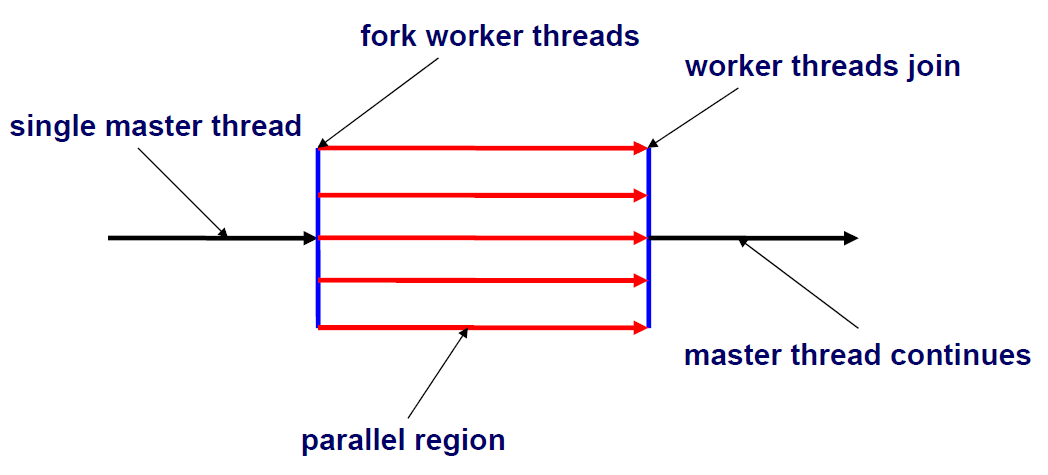
\includegraphics[width=\textwidth]{figures/openmp}
  \end{center}
\end{frame}

\begin{frame}{Parallel Control Structures}
  \begin{itemize}
  \item Two kinds of parallel constructs
    \begin{itemize}
    \item Create multiple threads (parallel directive)
    \item Divide work between an existing set of threads
    \end{itemize}
  \item Parallel directive
    \begin{itemize}
    \item Start a parallel region
    \end{itemize}
  \item For directive
    \begin{itemize}
    \item Exploit data-level parallelism (parallelize loops)
    \end{itemize}
  \item Sections directive
    \begin{itemize}
    \item Exploit thread-level parallelism (parallelize tasks)
    \end{itemize}
  \item Task directive (OpenMP 3.0)
    \begin{itemize}
    \item Task with ordering (not possible with sections)
    \end{itemize}
  \end{itemize}
\end{frame}

\begin{frame}{Communication \& Data Environment}
  \begin{itemize}
  \item Master thread (MT) exists the entire execution
  \item MT encounters a parallel construct
    \begin{itemize}
    \item Create a set of worker threads
    \item Stack is private to each thread
    \end{itemize}
  \item Data Scoping
    \begin{itemize}
    \item Shared variable: single storage location
    \item Private variable: multiple storage locations (1 per thread)
    \end{itemize}
  \end{itemize}
\end{frame}

\begin{frame}{Synchronization}
  \begin{itemize}
  \item Co-ordination of execution of multiple threads
  \item Critical directive: implement mutual exclusion
    \begin{itemize}
    \item Exclusive access for a single thread
    \end{itemize}
  \item Barrier directive: event synchronization
    \begin{itemize}
    \item Signal the occurrence of an event
    \end{itemize}
  \end{itemize}
\end{frame}

\begin{frame}[fragile]{Exploiting Loop-Level Parallelism}
  \begin{itemize}
  \item Important: program correctness
  \item Data dependencies:
    \begin{itemize}
    \item If two threads read from the same location and at least one
      thread writes to that location
      \begin{itemize}
      \item[$\rightarrow$] Data dependence
      \end{itemize}
    \item Example:
\begin{lstlisting}
for (i = 1; i < N; i++)
  a[i] = a[i] + a[i-1];
\end{lstlisting}
      \alert{Loop~carried~dependence}
    \end{itemize}
  \end{itemize}
\end{frame}

\begin{frame}[fragile]{Examples}
  \begin{tabular}{l r}
\begin{lstlisting}
for (i = 2; i <= n; i+= 2)
  a[i] = a[i] + a[i-1]
\end{lstlisting} & \pause\color{green}{No dependence}\pause \\[3em]
\begin{lstlisting}
for (i = 1; i <= n/2; i++)
  a[i] = a[i] + a[i + n/2]
\end{lstlisting} & \pause\color{green}{No dependence}\pause\\[3em]
\begin{lstlisting}
for (i = 1; i <= n/2 + 1; i++)
  a[i] = a[i] + a[i + n/2]
\end{lstlisting} & \pause\alert{Dependence:} \\
    & \alert{\lstinline!read(1+n/2)!} \\
    & \alert{\lstinline!write(n/2+1)!} \\
  \end{tabular}
\end{frame}

\begin{frame}[fragile]{Parallel Directive}
\begin{lstlisting}
//omp parallel shared (a,b) private (c,d)
\end{lstlisting}

  \vspace{\stretch{1}}

  \begin{itemize}
  \item Starts a parallel region
  \item \verb!shared!: variable is shared across all threads
  \item \verb!private!: each thread maintains a private copy
  \end{itemize}
\end{frame}

\begin{frame}[fragile]{Distribute Loop Iterations}
\begin{lstlisting}
//omp for schedule(dynamic)
\end{lstlisting}

\begin{lstlisting}
//omp for schedule(static)
\end{lstlisting}

  \vspace{\stretch{1}}

  \begin{itemize}
  \item Distribute loop iterations to worker threads
  \item \verb!dynamic!: loop-chunks are assigned to threads at runtime
  \item \verb!static!: loop-chunk assignment before the loop is
    executed
  \end{itemize}
\end{frame}

\begin{frame}[fragile]{Critical Section}
\begin{lstlisting}
//omp critical
\end{lstlisting}

  \vspace{\stretch{1}}

  \begin{itemize}
  \item Starts a critical section
  \item Code section is executed by a single thread at a time
  \end{itemize}
\end{frame}


\section{OpenMP in Java}

\begin{frame}{Outline}
  \tableofcontents[current]
\end{frame}

\begin{frame}{JOMP}
  \begin{itemize}
  \item Not natively supported by Java
  \item JOMP: source to source compiler
  \item TODO: More information (Wikipedia)
  \end{itemize}
\end{frame}

\begin{frame}{How to use on the Console}
  \begin{itemize}
  \item Download jar file from course page
  \item Import external JAR file to your project (classpath)
    \begin{itemize}
    \item \lstinline!export CLASSPATH=$\$$CLASSPATH:/path/to/jomp1.0b.jar!
    \item Use option \lstinline!-cp /path/to/jomp1.0b.jar! when
      calling Java to transform \lstinline!file.jomp! into
      \lstinline!file.java!
    \end{itemize}
  \item Perform the following steps in the console
    \begin{itemize}
    \item \lstinline!java jomp.compiler.Jomp file.jomp!
      \begin{itemize}
      \item[$\rightarrow$] generates \lstinline!file.java!
      \end{itemize}
    \item \lstinline!javac file.java!
    \item \lstinline!java file!
    \end{itemize}
  \end{itemize}
\end{frame}

\begin{frame}{How to use in Eclipse}
  TODO
\end{frame}


\section{Assignment 10}

\begin{frame}{Outline}
  \tableofcontents[current]
\end{frame}

\begin{frame}{Tasks}
  Task 1
  \begin{itemize}
  \item Parallelize an existing implementation with OpenMP
  \item Which loop nest would you parallelize?
  \item Do you need a critical section?
  \end{itemize}

  \vspace{\stretch{1}}

  Task 2
  \begin{itemize}
  \item Implement a Block Matrix Multiplication
  \item Divide the source matrices into sub-matrices
  \item Assign a thread to each sub-matrix
  \end{itemize}

  \vspace{\stretch{1}}

  Which one performs better?
\end{frame}


\section*{Outro}

\begin{frame}{Summary}
  \begin{itemize}
  \item TODO
  \end{itemize}
\end{frame}

\end{document}
